%% ----------------------------------------------------------------
%% Introduction.tex
%% ---------------------------------------------------------------- 
\chapter{Introduction} \label{Chapter:Introduction}
%The Introduction to my Report \dots

%The initial idea of the project was taken from Pirobot(\cite{Pirobot}).
%
%\inote{what it will do. Define everything. Use. Very general}
%General - mapping robots. 
%
%stereovision - uses etc.
%
%other similar projects
%
%why mine is important 

%\inote{Talk about what I set out to do, include some definitions etc. }
%\inote{What I ended up doing}
%\inote{The uses of my robot.} 

The original idea for the project was a stereoscopic mapping robot, similar to \cite{Pirobot}. This would autonomously search an area and return an occupancy map \citep{thrun2003learning}. However, due to time constraints, the image processing aspects remain prototyped in MATLAB, but not implemented in C. The end robot is able to capture stereo image pairs, move with reasonable accuracy and compute Fourier Transforms. The robot can run a predefined set of commands automatically or act as a shell terminal.

Stereoscopy in computer vision is the ability to calculate the locations and depths using images from two or more cameras, which are used to triangulate and estimate distances \citep{Saxena:DepthEstimation}. By using two cameras on the same plane, separated by a set horizontal distance, the depth of the observed scene can be perceived by the system.

Stereo vision is a small section of computer vision which is widely used in many applications. Microsoft's Xbox Kinect \citep{Microsoft:Kinect} uses stereo vision to locate a game player in order to use their movements to control the game. \cite{Mrovlje:Distance_Stereoscopic} uses stereo vision to be able to locate the distance to a marker. 
\inote{Leap Motion?}
The stereo vision robot discussed in this report is a low cost alternative to other robots which use laser range finders or high quality cameras \citep{Se:MappingRobot}. The robot was mounted on the base seen in figure \ref{fig:RobotBase} and used two OmniVision OV7670 cameras delivering QVGA format images.

The final robot designed could be used for a variety of applications. The robot can perceive depth of the captured area so can avoid obstacles and navigate. The robot could also be adapted to stream the camera data to a remote computer and be controlled by a user to explore unknown and potentially hostile areas safely. 

\begin{figure}
\centering
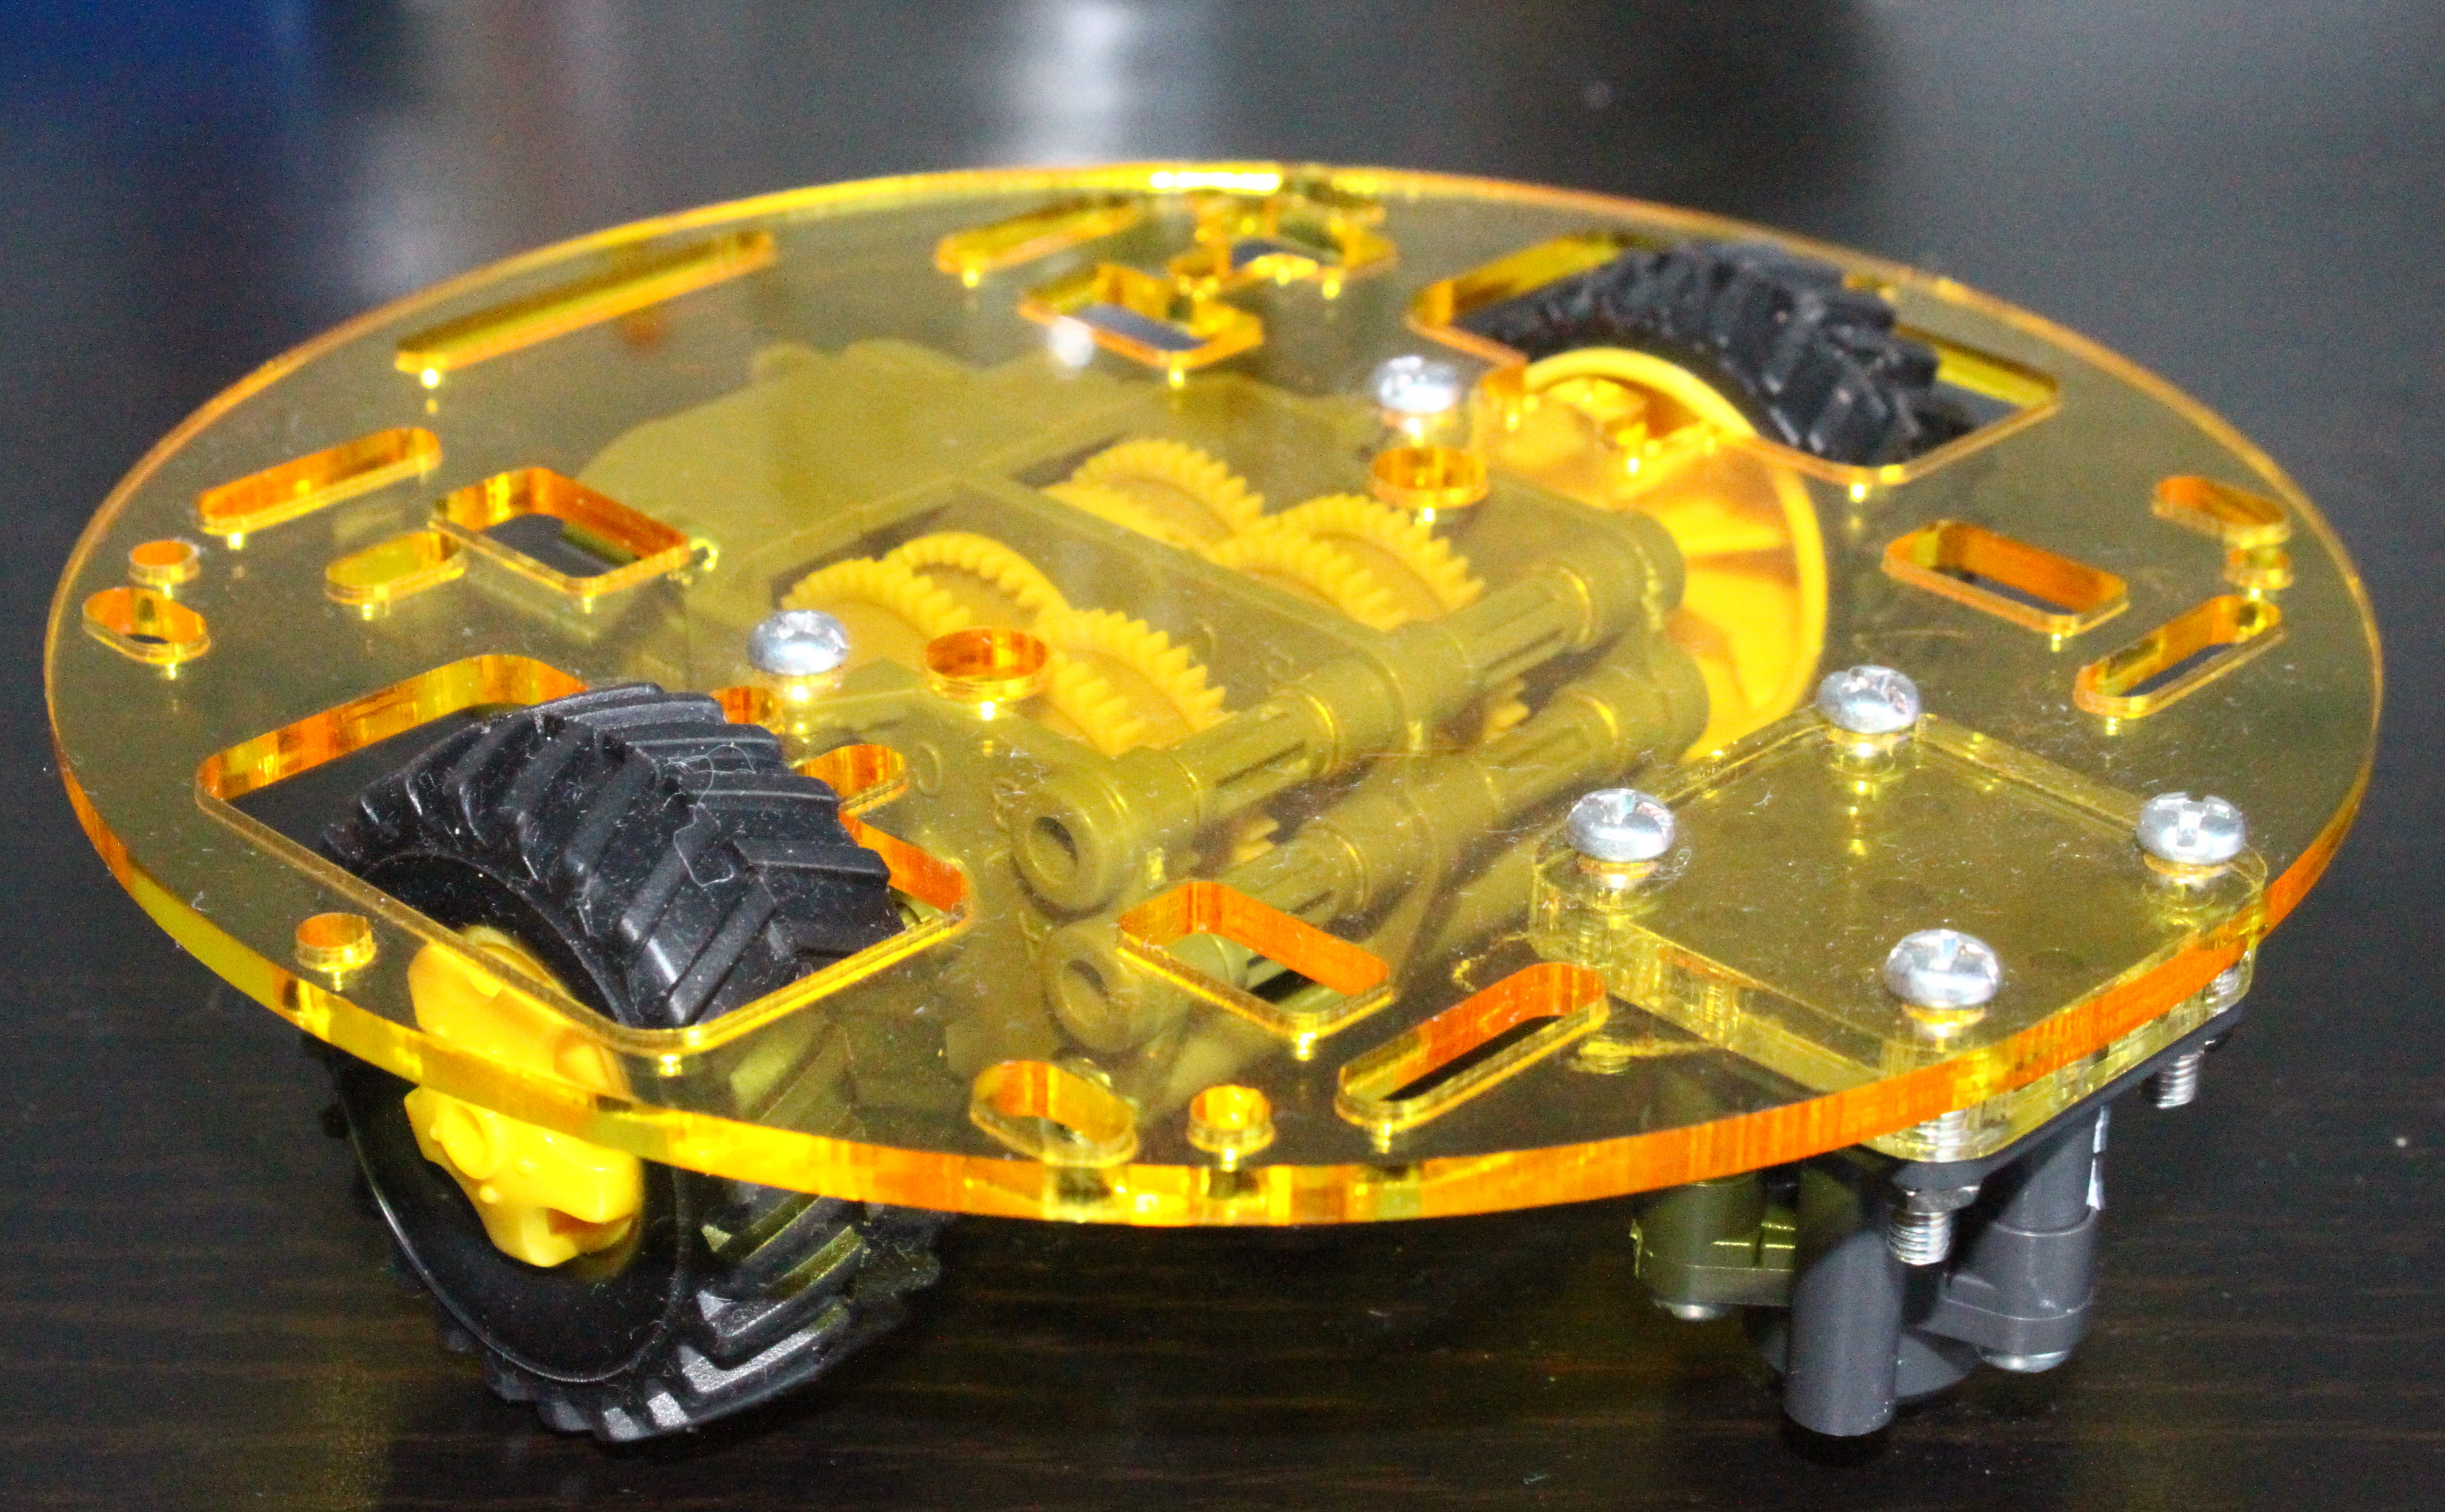
\includegraphics[width=\textwidth - 2cm]{./Figures/RobotBase.jpg}
\caption{The base of the robot}
\label{fig:RobotBase}
\end{figure}

\section{Project Management}
In order to reduce the risk within the project, all aspects of potential issues were looked at and are summarised in table \ref{tab:risk}. A Gantt chart of how time was planned to be spent can be seen in figure \ref{fig:Gantt}.  

The project was designed in stages - first, gaining operation of all the basic sections; movement, image capturing, image detection algorithms etc. These were then be brought together once tested to create the final product. This meant functionality was obtained of the basic aspects before addressing more complex issues. 
\begin{table}
\begin{tabular}{p{6cm}p{2cm}p{6cm}}\toprule
Risk						&	Severity	&	Prevention \\ \toprule
Components not arriving on time	&	High		&	Order parts as early as possible \\ \midrule
Project not fulfilling specification				&	High		&	Develop in stages to obtain functionality in parts. Ensure enough time is allocated to the project.	\\\midrule
PCB Design is incorrect		&	Medium		&	Check the design carefully and get second opinion. \\\midrule
Failure of personal computer causing data loss & Low	& 	Keep back ups of all work on Devtrack Git repository and Dropbox.\\

\bottomrule
\end{tabular}
\caption{A list of risks and the prevention steps taken to reduce their impact}
\label{tab:risk}
\end{table}
